In this section we show results of our program. The program is opensource (BSD
licensed) and available at \url{http://sfepy.org}, use the release 00.50.00 to
get the exact results as below.

\section{Solution of the Schr\"odinger Equation}

The first thing we need to do is to create a mesh.

\subsection{2D: Mesh}

We create a mesh:

\begin{lstlisting}
$ ./schroedinger.py --mesh --2d
Dimension: 2
Info    : 'gmsh -2 tmp/mesh.geo -format mesh' started on Sat Jul 19 02:04:41 2008
Info    : Reading 'tmp/mesh.geo'
Info    : Read 'tmp/mesh.geo'
Info    : Meshing 1D...
Info    : Meshing curve 1 (Line)
Info    : Meshing curve 2 (Line)
Info    : Meshing curve 3 (Line)
Info    : Meshing curve 4 (Line)
Info    : Mesh 1D complete (0.028002 s)
Info    : Mesh
Info    : Meshing 2D...
Info    : Meshing surface 6 (Plane, MeshAdapt+Delaunay)
Info    : Mesh 2D complete (3.65223 s)
Info    : Mesh
Info    : 8100 vertices 16198 elements
Info    : Writing 'tmp/mesh.mesh'
Info    : Wrote 'tmp/mesh.mesh'
Mesh written to tmp/mesh.vtk
\end{lstlisting}

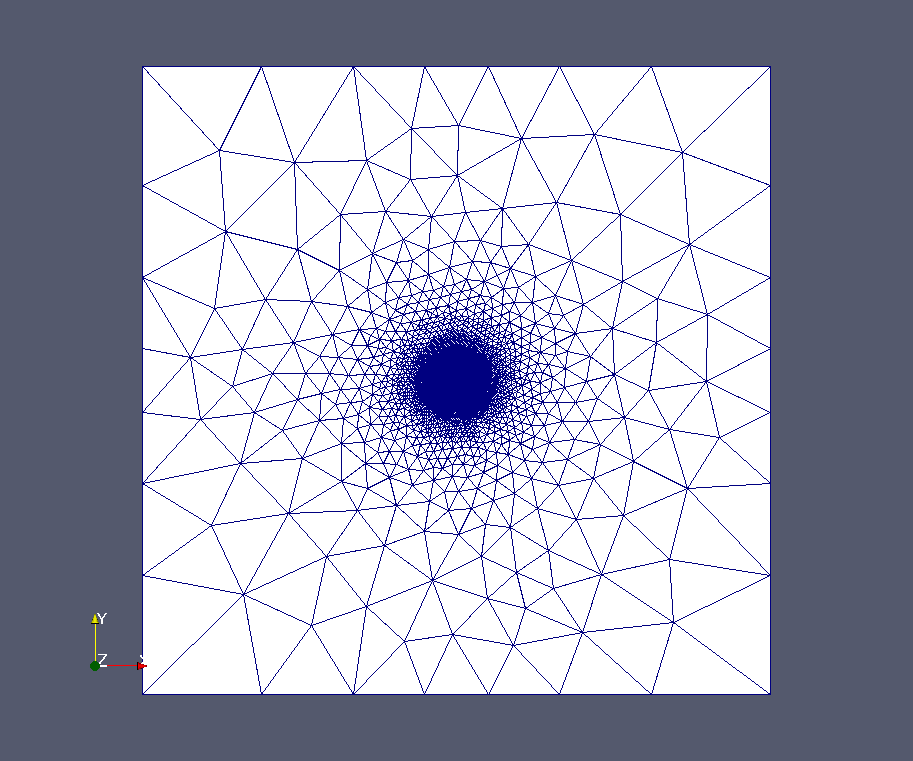
\includegraphics[width=12cm]{images/mesh1.png}

\subsection{2D: Potential Well}

This is also sometimes called particle in the box.

\begin{lstlisting}
$ ./schroedinger.py --well
Dimension: 2
sfepy: left over: ['tau', 'n_eigs', 'mesh', 'quadr', 'dim', 'base_approx']
sfepy: reading mesh (tmp/mesh.vtk)...
sfepy: ...done in 0.37 s
sfepy: setting up domain edges...
sfepy: ...done in 0.10 s
sfepy: creating regions...
sfepy:     leaf Omega region_1000
sfepy:     leaf Surface region_2
sfepy: ...done in 0.11 s
sfepy: equation "rhs":
sfepy: dw_mass_scalar.i1.Omega( v, Psi )
sfepy: equation "lhs":
sfepy:   dw_laplace.i1.Omega( m.val, v, Psi )
                   + dw_mass_scalar_variable.i1.Omega( matV.V, v, Psi )
sfepy: describing geometries...
sfepy: ...done in 0.02 s
sfepy: setting up dof connectivities...
sfepy: ...done in 0.00 s
sfepy: matrix shape: (8072, 8072)
sfepy: assembling matrix graph...
sfepy: ...done in 0.02 s
sfepy: matrix structural nonzeros: 56442 (8.66e-04% fill)
sfepy: updating materials...
sfepy:     m
sfepy:     matV
sfepy: ...done in 0.00 s
sfepy: assembling lhs...
sfepy:   setting up dof connectivities...
sfepy:   ...done in 0.00 s
sfepy: ...done in 0.04 s
sfepy: assembling rhs...
sfepy:   setting up dof connectivities...
sfepy:   ...done in 0.00 s
sfepy: ...done in 0.02 s
computing resonance frequencies...
sfepy: loading...
sfepy: ...done
sfepy: solving...
sfepy:   number of converged eigenvalues: 10
sfepy: ...done in 3.10 s
sfepy: reading mesh (tmp/mesh.vtk)...
sfepy: ...done in 0.42 s
a=100.000000
Energies:
n      exact         FEM      error
0:  0.00098696   0.00100813   2.14%
1:  0.00246740   0.00255738   3.65%
2:  0.00246740   0.00256454   3.94%
3:  0.00394784   0.00421025   6.65%
4:  0.00493480   0.00524481   6.28%
5:  0.00493480   0.00525660   6.52%
6:  0.00641524   0.00705958  10.04%
7:  0.00641524   0.00706794  10.17%
8:  0.00838916   0.00916761   9.28%
9:  0.00838916   0.00920827   9.76%
Solution saved to mesh.vtk
\end{lstlisting}

\subsection{2D: Linear Harmonic Oscillator}

\begin{lstlisting}
$ ./schroedinger.py --oscillator
Dimension: 2
sfepy: left over: ['tau', 'n_eigs', 'mesh', 'quadr', 'dim', 'base_approx']
sfepy: reading mesh (tmp/mesh.vtk)...
sfepy: ...done in 0.36 s
sfepy: setting up domain edges...
sfepy: ...done in 0.10 s
sfepy: creating regions...
sfepy:     leaf Omega region_1000
sfepy:     leaf Surface region_2
sfepy: ...done in 0.08 s
sfepy: equation "rhs":
sfepy: dw_mass_scalar.i1.Omega( v, Psi )
sfepy: equation "lhs":
sfepy:   dw_laplace.i1.Omega( m.val, v, Psi )
                   + dw_mass_scalar_variable.i1.Omega( matV.V, v, Psi )
sfepy: describing geometries...
sfepy: ...done in 0.01 s
sfepy: setting up dof connectivities...
sfepy: ...done in 0.00 s
sfepy: matrix shape: (8072, 8072)
sfepy: assembling matrix graph...
sfepy: ...done in 0.02 s
sfepy: matrix structural nonzeros: 56442 (8.66e-04% fill)
sfepy: updating materials...
sfepy:     m
sfepy:     matV
sfepy: ...done in 0.00 s
sfepy: assembling lhs...
sfepy:   setting up dof connectivities...
sfepy:   ...done in 0.00 s
sfepy: ...done in 0.03 s
sfepy: assembling rhs...
sfepy:   setting up dof connectivities...
sfepy:   ...done in 0.00 s
sfepy: ...done in 0.02 s
computing resonance frequencies...
sfepy: loading...
sfepy: ...done
sfepy: solving...
sfepy:   number of converged eigenvalues: 16
sfepy: ...done in 7.38 s
sfepy: reading mesh (tmp/mesh.vtk)...
sfepy: ...done in 0.36 s
a=100.000000
Energies:
n      exact         FEM      error
0:  1.00000000   1.00081703   0.08%
1:  2.00000000   2.00158339   0.08%
2:  2.00000000   2.00175346   0.09%
3:  3.00000000   3.00302269   0.10%
4:  3.00000000   3.00334897   0.11%
5:  3.00000000   3.00346025   0.12%
6:  4.00000000   4.00498898   0.12%
7:  4.00000000   4.00571512   0.14%
8:  4.00000000   4.00606336   0.15%
9:  4.00000000   4.00631703   0.16%
10:  5.00000000   5.00743227   0.15%
11:  5.00000000   5.00868813   0.17%
12:  5.00000000   5.00947456   0.19%
13:  5.00000000   5.01031228   0.21%
14:  5.00000000   5.01042976   0.21%
15:  6.00000000   6.01161255   0.19%
Solution saved to mesh.vtk
\end{lstlisting}

\subsection{2D: Hydrogen Atom}

\begin{lstlisting}
$ ./schroedinger.py --hydrogen
Dimension: 2
sfepy: left over: ['tau', 'n_eigs', 'mesh', 'quadr', 'dim', 'base_approx']
sfepy: reading mesh (tmp/mesh.vtk)...
sfepy: ...done in 0.38 s
sfepy: setting up domain edges...
sfepy: ...done in 0.08 s
sfepy: creating regions...
sfepy:     leaf Omega region_1000
sfepy:     leaf Surface region_2
sfepy: ...done in 0.10 s
sfepy: equation "rhs":
sfepy: dw_mass_scalar.i1.Omega( v, Psi )
sfepy: equation "lhs":
sfepy:   dw_laplace.i1.Omega( m.val, v, Psi )
                   + dw_mass_scalar_variable.i1.Omega( matV.V, v, Psi )
sfepy: describing geometries...
sfepy: ...done in 0.01 s
sfepy: setting up dof connectivities...
sfepy: ...done in 0.01 s
sfepy: matrix shape: (8072, 8072)
sfepy: assembling matrix graph...
sfepy: ...done in 0.01 s
sfepy: matrix structural nonzeros: 56442 (8.66e-04% fill)
sfepy: updating materials...
sfepy:     m
sfepy:     matV
sfepy: ...done in 0.01 s
sfepy: assembling lhs...
sfepy:   setting up dof connectivities...
sfepy:   ...done in 0.00 s
sfepy: ...done in 0.03 s
sfepy: assembling rhs...
sfepy:   setting up dof connectivities...
sfepy:   ...done in 0.00 s
sfepy: ...done in 0.02 s
computing resonance frequencies...
sfepy: loading...
sfepy: ...done
sfepy: solving...
sfepy:   number of converged eigenvalues: 10
sfepy: ...done in 10.35 s
sfepy: reading mesh (tmp/mesh.vtk)...
sfepy: ...done in 0.43 s
a=100.000000
Energies:
n      exact         FEM      error
0:  -0.50000000   -0.48444312   3.11%
1:  -0.05555556   -0.05546226   0.17%
2:  -0.05555556   -0.05490833   1.17%
3:  -0.02000000   -0.01987759   0.61%
4:  -0.02000000   -0.01986552   0.67%
5:  -0.02000000   -0.01978261   1.09%
6:  -0.02000000   -0.01974034   1.30%
7:  -0.02000000   -0.01973349   1.33%
8:  -0.01020408   -0.00961296   5.79%
9:  -0.01020408   -0.00959015   6.02%
Solution saved to mesh.vtk
\end{lstlisting}

\subsection{2D: Boron Atom}

\begin{lstlisting}
$ ./schroedinger.py --boron
[...]
Energies:
n      exact         FEM      error
0:  -12.50000000   -12.65582408   1.25%
1:  -1.38888889   -1.39403240   0.37%
2:  -1.38888889   -1.38823512   0.05%
3:  -1.38888889   -1.38821053   0.05%
4:  -0.50000000   -0.50042416   0.08%
5:  -0.50000000   -0.49898923   0.20%
6:  -0.50000000   -0.49895079   0.21%
7:  -0.50000000   -0.49809201   0.38%
8:  -0.50000000   -0.49804906   0.39%
9:  -0.25510204   -0.25394635   0.45%
10:  -0.25510204   -0.25329618   0.71%
11:  -0.25510204   -0.25324683   0.73%
12:  -0.25510204   -0.25249085   1.02%
13:  -0.25510204   -0.25242286   1.05%
Solution saved to mesh.vtk
\end{lstlisting}

\subsection{3D: Mesh}

\begin{lstlisting}
$ ./schroedinger.py --mesh
Dimension: 3
Info    : 'gmsh -0 database/box.geo -o tmp/x.geo' started on Sat Jul 19 02:08:14 2008
Info    : Reading 'database/box.geo'
Info    : Read 'database/box.geo'
Info    : Writing 'tmp/x.geo'
Info    : Wrote 'tmp/x.geo'
General geometry information:
  points: 8
  lines: 12
  surfaces: 6
  volumes: 1
Physical entities:
  surfaces (boundary conditions):
  volumes (regions):
    1: volume numbers [1]
Generating mesh using /usr/bin/tetgen -pQAq1.000000 -a0.030000 tmp/t.poly
sfepy: reading mesh (tmp/t.1.node)...
       nodes: 100% |############################################| Time: 00:00:00
       elements: 100% |#########################################| Time: 00:00:01
sfepy: ...done in 1.39 s
Mesh written to tmp/mesh.vtk
\end{lstlisting}

\subsection{3D: Potential Well}

\begin{lstlisting}
$ ./schroedinger.py --well
Dimension: 3
sfepy: left over: ['tau', 'n_eigs', 'mesh', 'quadr', 'dim', 'base_approx']
sfepy: reading mesh (tmp/mesh.vtk)...
sfepy: ...done in 1.24 s
sfepy: setting up domain edges...
sfepy: ...done in 0.89 s
sfepy: setting up domain faces...
sfepy: ...done in 0.66 s
sfepy: creating regions...
sfepy:     leaf Omega region_1000
sfepy:     leaf Surface region_2
sfepy: ...done in 1.01 s
sfepy: equation "rhs":
sfepy: dw_mass_scalar.i1.Omega( v, Psi )
sfepy: equation "lhs":
sfepy:   dw_laplace.i1.Omega( m.val, v, Psi )
                   + dw_mass_scalar_variable.i1.Omega( matV.V, v, Psi )
sfepy: describing geometries...
sfepy: ...done in 0.15 s
sfepy: setting up dof connectivities...
sfepy: ...done in 0.01 s
sfepy: matrix shape: (7964, 7964)
sfepy: assembling matrix graph...
sfepy: ...done in 0.09 s
sfepy: matrix structural nonzeros: 117024 (1.85e-03% fill)
sfepy: updating materials...
sfepy:     m
sfepy:     matV
sfepy: ...done in 0.00 s
sfepy: assembling lhs...
sfepy:   setting up dof connectivities...
sfepy:   ...done in 0.01 s
sfepy: ...done in 0.20 s
sfepy: assembling rhs...
sfepy:   setting up dof connectivities...
sfepy:   ...done in 0.01 s
sfepy: ...done in 0.08 s
computing resonance frequencies...
sfepy: loading...
sfepy: ...done
sfepy: solving...
sfepy:   number of converged eigenvalues: 20
sfepy: ...done in 5.47 s
sfepy: reading mesh (tmp/mesh.vtk)...
sfepy: ...done in 1.13 s
a=10.000000
Energies:
n      exact         FEM      error
0:  0.14804407   0.14922535   0.80%
1:  0.29608813   0.30079010   1.59%
2:  0.29608813   0.30082698   1.60%
3:  0.29608813   0.30084093   1.61%
4:  0.44413220   0.45473187   2.39%
5:  0.44413220   0.45482735   2.41%
6:  0.44413220   0.45489304   2.42%
7:  0.54282824   0.55869467   2.92%
8:  0.54282824   0.55871268   2.93%
9:  0.54282824   0.55889291   2.96%
10:  0.59217626   0.61113461   3.20%
11:  0.69087231   0.71656267   3.72%
12:  0.69087231   0.71661781   3.73%
13:  0.69087231   0.71678728   3.75%
14:  0.69087231   0.71695827   3.78%
15:  0.69087231   0.71706618   3.79%
16:  0.69087231   0.71729282   3.82%
17:  0.83891637   0.87708704   4.55%
18:  0.83891637   0.87715932   4.56%
19:  0.83891637   0.87797932   4.66%
Solution saved to mesh.vtk

\end{lstlisting}

\subsection{3D: Linear Harmonic Oscillator}

\begin{lstlisting}
$ ./schroedinger.py --oscillator
Dimension: 3
sfepy: left over: ['tau', 'n_eigs', 'mesh', 'quadr', 'dim', 'base_approx']
sfepy: reading mesh (tmp/mesh.vtk)...
sfepy: ...done in 1.31 s
sfepy: setting up domain edges...
sfepy: ...done in 0.96 s
sfepy: setting up domain faces...
sfepy: ...done in 0.73 s
sfepy: creating regions...
sfepy:     leaf Omega region_1000
sfepy:     leaf Surface region_2
sfepy: ...done in 1.19 s
sfepy: equation "rhs":
sfepy: dw_mass_scalar.i1.Omega( v, Psi )
sfepy: equation "lhs":
sfepy:   dw_laplace.i1.Omega( m.val, v, Psi )
                   + dw_mass_scalar_variable.i1.Omega( matV.V, v, Psi )
sfepy: describing geometries...
sfepy: ...done in 0.18 s
sfepy: setting up dof connectivities...
sfepy: ...done in 0.00 s
sfepy: matrix shape: (7964, 7964)
sfepy: assembling matrix graph...
sfepy: ...done in 0.12 s
sfepy: matrix structural nonzeros: 117024 (1.85e-03% fill)
sfepy: updating materials...
sfepy:     m
sfepy:     matV
sfepy: ...done in 0.00 s
sfepy: assembling lhs...
sfepy:   setting up dof connectivities...
sfepy:   ...done in 0.00 s
sfepy: ...done in 0.24 s
sfepy: assembling rhs...
sfepy:   setting up dof connectivities...
sfepy:   ...done in 0.00 s
sfepy: ...done in 0.10 s
computing resonance frequencies...
sfepy: loading...
sfepy: ...done
sfepy: solving...
sfepy:   number of converged eigenvalues: 20
sfepy: ...done in 3.96 s
sfepy: reading mesh (tmp/mesh.vtk)...
sfepy: ...done in 1.33 s
a=10.000000
Energies:
n      exact         FEM      error
0:  1.50000000   1.60246586   6.83%
1:  2.50000000   2.66350384   6.54%
2:  2.50000000   2.66592179   6.64%
3:  2.50000000   2.66745129   6.70%
4:  3.50000000   3.73764474   6.79%
5:  3.50000000   3.74251455   6.93%
6:  3.50000000   3.74545592   7.01%
7:  3.50000000   3.74824003   7.09%
8:  3.50000000   3.75739243   7.35%
9:  3.50000000   3.78188467   8.05%
10:  4.50000000   4.84098311   7.58%
11:  4.50000000   4.84411120   7.65%
12:  4.50000000   4.84695596   7.71%
13:  4.50000000   4.85068992   7.79%
14:  4.50000000   4.85439463   7.88%
15:  4.50000000   4.86152828   8.03%
16:  4.50000000   4.86513080   8.11%
17:  4.50000000   4.91355134   9.19%
18:  4.50000000   4.91666221   9.26%
19:  4.50000000   4.92487984   9.44%
Solution saved to mesh.vtk
\end{lstlisting}

\subsection{3D: Hydrogen Atom}

\begin{lstlisting}
$ ./schroedinger.py --hydrogen
Dimension: 3
sfepy: left over: ['tau', 'n_eigs', 'mesh', 'quadr', 'dim', 'base_approx']
sfepy: reading mesh (tmp/mesh.vtk)...
sfepy: ...done in 1.18 s
sfepy: setting up domain edges...
sfepy: ...done in 0.83 s
sfepy: setting up domain faces...
sfepy: ...done in 0.67 s
sfepy: creating regions...
sfepy:     leaf Omega region_1000
sfepy:     leaf Surface region_2
sfepy: ...done in 0.98 s
sfepy: equation "rhs":
sfepy: dw_mass_scalar.i1.Omega( v, Psi )
sfepy: equation "lhs":
sfepy:   dw_laplace.i1.Omega( m.val, v, Psi )
                   + dw_mass_scalar_variable.i1.Omega( matV.V, v, Psi )
sfepy: describing geometries...
sfepy: ...done in 0.15 s
sfepy: setting up dof connectivities...
sfepy: ...done in 0.00 s
sfepy: matrix shape: (7964, 7964)
sfepy: assembling matrix graph...
sfepy: ...done in 0.09 s
sfepy: matrix structural nonzeros: 117024 (1.85e-03% fill)
sfepy: updating materials...
sfepy:     m
sfepy:     matV
sfepy: ...done in 0.00 s
sfepy: assembling lhs...
sfepy:   setting up dof connectivities...
sfepy:   ...done in 0.00 s
sfepy: ...done in 0.19 s
sfepy: assembling rhs...
sfepy:   setting up dof connectivities...
sfepy:   ...done in 0.00 s
sfepy: ...done in 0.08 s
computing resonance frequencies...
sfepy: loading...
sfepy: ...done
sfepy: solving...
sfepy:   number of converged eigenvalues: 5
sfepy: ...done in 1.11 s
sfepy: reading mesh (tmp/mesh.vtk)...
sfepy: ...done in 1.31 s
a=10.000000
Energies:
n      exact         FEM      error
0:  -0.50000000   -0.13468961  73.06%
1:  -0.12500000   0.13909268  211.27%
2:  -0.12500000   0.13934116  211.47%
3:  -0.12500000   0.13939501  211.52%
4:  -0.12500000   0.26835117  314.68%
Solution saved to mesh.vtk
\end{lstlisting}

\subsection{2D: nonsymmetric potential I}

In this example we use a potential from two nuclei positioned at $(-5, 0)$ and
$(5, 0)$. This is a nonsymmetric problem, thus one cannot use the usual
way to reduce the Schr\"odinger equation to radial and angular
parts. A general partial differential equations solver (in our case FEM) has to
be used.

\subsection{2D: nonsymmetric potential II}

In this example we use a potential from three nuclei positioned at $(-5, 0)$,
$(5, 0)$ and $(0, 5)$.

\section{Density Functional Theory, Spherically Symmetric Solution}

\subsection{Pb: LDA}

\begin{lstlisting}
0: |F(x)|=32381.03274296
1: |F(x)|=5347.06647460
2: |F(x)|=2283.82989218
3: |F(x)|=148.26174998
4: |F(x)|=120.78098800
5: |F(x)|=84.68248231
6: |F(x)|=11.30008638
7: |F(x)|=3.65004163
8: |F(x)|=3.12545615
9: |F(x)|=1.44414848
10: |F(x)|=0.32879840
11: |F(x)|=0.10891716
12: |F(x)|=0.03456829
13: |F(x)|=0.01240870
14: |F(x)|=0.00774382
15: |F(x)|=0.00302906
16: |F(x)|=0.00081825
17: |F(x)|=0.00026270
18: |F(x)|=0.00007814
19: |F(x)|=0.00003516
1s( 2) j=l+1/2: -2901.078061
2s( 2) j=l+1/2: -488.8433352
2p( 6) j=l+1/2: -470.8777849
3s( 2) j=l+1/2: -116.526852
3p( 6) j=l+1/2: -107.950391
3d(10) j=l+1/2: -91.88992429
4s( 2) j=l+1/2: -25.75333021
4p( 6) j=l+1/2: -21.99056413
4d(10) j=l+1/2: -15.03002657
4f(14) j=l+1/2: -5.592531664
5s( 2) j=l+1/2: -4.206797624
5p( 6) j=l+1/2: -2.941656967
5d(10) j=l+1/2: -0.9023926829
6s( 2) j=l+1/2: -0.3571868295
6p( 2) j=l+1/2: -0.1418313263
\end{lstlisting}

This is agrees with the NIST reference calculation to all decimal digits.

\subsection{Pb: RLDA}

\begin{lstlisting}
0: |F(x)|=41056.67822797
1: |F(x)|=7926.04357205
2: |F(x)|=2858.46358638
3: |F(x)|=598.63802038
4: |F(x)|=268.50208068
5: |F(x)|=30.05744371
6: |F(x)|=27.56292000
7: |F(x)|=11.22084649
8: |F(x)|=4.78645898
9: |F(x)|=0.53300950
10: |F(x)|=0.13956963
11: |F(x)|=0.07821891
12: |F(x)|=0.06505839
13: |F(x)|=0.02021479
14: |F(x)|=0.00240256
15: |F(x)|=0.00132181
16: |F(x)|=0.00079552
17: |F(x)|=0.00018579
18: |F(x)|=0.00000838
19: |F(x)|=0.00000584
1s( 2) j=l+1/2: -3209.51946
2s( 2) j=l+1/2: -574.1825655
2p( 6) j=l-1/2: -551.7234408
2p( 6) j=l+1/2: -472.3716103
3s( 2) j=l+1/2: -137.8642241
3p( 6) j=l-1/2: -127.6789451
3p( 6) j=l+1/2: -109.9540395
3d(10) j=l-1/2: -93.15817605
3d(10) j=l+1/2: -89.36399096
4s( 2) j=l+1/2: -31.15015728
4p( 6) j=l-1/2: -26.73281564
4p( 6) j=l+1/2: -22.38230707
4d(10) j=l-1/2: -15.1647618
4d(10) j=l+1/2: -14.3484973
5s( 2) j=l+1/2: -5.225938506
4f(14) j=l-1/2: -4.960490099
4f(14) j=l+1/2: -4.775660273
5p( 6) j=l-1/2: -3.710458943
5p( 6) j=l+1/2: -2.889127431
5d(10) j=l-1/2: -0.8020049565
5d(10) j=l+1/2: -0.7070299184
6s( 2) j=l+1/2: -0.4209603386
6p( 2) j=l-1/2: -0.1549640727
\end{lstlisting}

This is agrees within $12\%$ to the NIST reference calculation, the difference
being caused probably by a different exchange and correlation potential
approximation in our code in NIST.

\subsection{B: LDA}

\begin{lstlisting}
1:  |F(x)|=467.33470427
2:  |F(x)|=39.46088238
3:  |F(x)|=5.59717305
4:  |F(x)|=3.09300726
5:  |F(x)|=2.04909614
6:  |F(x)|=0.09754169
7:  |F(x)|=0.06773803
8:  |F(x)|=0.04587578
9:  |F(x)|=0.00592044
10:  |F(x)|=0.00382678
11:  |F(x)|=0.00232014
12:  |F(x)|=0.00005561
13:  |F(x)|=0.00002714
14:  |F(x)|=0.00001809
15:  |F(x)|=0.00000042
16:  |F(x)|=0.00000023
17:  |F(x)|=0.00000014
18:  |F(x)|=0.00000001
19:  |F(x)|=0.00000000
20:  |F(x)|=0.00000000
1s( 2) j=l+1/2: -6.564347081
2s( 2) j=l+1/2: -0.3447010093
2p( 1) j=l+1/2: -0.1366031499
\end{lstlisting}

Agrees with NIST to all decimal places.

\subsection{B: RLDA}

\begin{lstlisting}
0: |F(x)|=485.06815695
1: |F(x)|=103.13739852
2: |F(x)|=34.94893789
3: |F(x)|=18.15071235
4: |F(x)|=1.19766447
5: |F(x)|=0.10974802
6: |F(x)|=0.07628667
7: |F(x)|=0.02450426
8: |F(x)|=0.00430650
9: |F(x)|=0.00193614
10: |F(x)|=0.00042938
11: |F(x)|=0.00010306
12: |F(x)|=0.00002872
13: |F(x)|=0.00001073
14: |F(x)|=0.00000217
15: |F(x)|=0.00000090
16: |F(x)|=0.00000028
17: |F(x)|=0.00000015
18: |F(x)|=0.00000002
19: |F(x)|=0.00000001
1s( 2) j=l+1/2: -6.56282977
2s( 2) j=l+1/2: -0.3447247582
2p( 1) j=l-1/2: -0.1366103284
\end{lstlisting}

Agrees with NIST to 3 decimal places after the decimal dot, the difference also
probably causes by a different exchange and correlation potential
approximation.
